\documentclass{article}
\usepackage{amsmath, amssymb}
\usepackage{cancel}
\usepackage{tikz}
\usepackage{mdframed}
\usepackage{hyperref}
\usetikzlibrary{automata, positioning, arrows}

\begin{document}

\section{Lecture 15: Plan for Class}
Last time:
\begin{enumerate}
    \item Melnikov's method
\end{enumerate}

Today:
\begin{enumerate}
    \item Melnikov revisited
    \item 1-d maps and symbolic dynamics
    \item Period-3 implies chaos
    \item Cantor sets and dynamics on them
\end{enumerate}

\section{Melnikov method}

\subsection{Time-period systems}
Melnikov's method usually is applied to time-periodic planar ($\mathbb{R}^2$) perturbations of Hamiltonian systems
\[
\dot{x} = f(x) + \epsilon g(x,t)
\]
where $f(x)$ is Hamiltonian and $g(x,t+T)=g(x,t)$ for all $x,t$. Suppose $\dot{x}=f(x)$ has a hyperbolic saddle with a homoclinic orbit $q(t)$. Now we are going to look at the Poincare map of the perturbed system.

\subsection{Melnikov function}

We can define the Melnikov function as 
\[
M(t_0) = \int_{-\infty}^{\infty}\left(f\times g\right)\left(q_0(t),t+t_0\right)dt
\]
where $\times$ is the cross product. Now, stable and unstable manifolds of the Poincare map intersect transversely if and only if $M$ has simple zeros.

\subsubsection{Geometric intuition}

Rowley is drawing a 3D picture of the homoclinic orbit as the time of the system unfolds over the period $T$. We're looking at a time slice $t_0$ and reasoning about the distance between the stable and unstable manifolds at point $q_0(t_0)$. As we vary $t_0$, the point at which we take the time slice, we want the distance between the stable and unstable manifold to decrease, cross zero, and then increase. This is a simple zero and shows that the manifolds intersect. The picture is clever.

\subsubsection{Nitty gritty}

We need to approximate the solutions in the stable and unstable manifolds of $\gamma_\epsilon(t)$. Via some lemma that Rowley mentioned, we have 
\[
q^s_\epsilon(t,t_0) = q_0(t,t_0) + \epsilon q_1^s (t,t_0) _ \mathcal{O}(\epsilon^2)
\]
which is valid for $t\in[t_0,\infty)$, and 
\[
q^u_\epsilon(t,t_0) = q_0(t,t_0) + \epsilon q_1^u (t,t_0) _ \mathcal{O}(\epsilon^2)
\]
which is valid for $t\in(-\infty, t_0]$. Also note that $q_0$ is the unperturbed orbit and $q_1$ is the perturbed orbit. We want to substitute these manifold approximations into our dynamics $\dot{x} = f(x) + \epsilon g(x,t)$ by writing
\begin{align*}
    \dot{q}_0&=f(q_0)\\
    \dot{q}_1&=Df(q_0(t-t_0))q^{s,u}_1+g(q_0(t-t_0),t)
\end{align*}
Now our signed distance function is 
\[
M(t_0) = f(q_0(0))\times \left(q^u_1(t_0,t_0)-q^s_1(t_0,t_0)\right)
\]
where the use of the cross product follows because 
\[
f^\bot\cdot q=(-f_2,f_1)\cdot(q_1,q_2)=f_1q_2 - f_2q_1 = f\times g
\]
meaning it's the dot product with $f^\bot$.

Alright so I got confused and couldn't keep up. Here are the rest of the notes transcribed by Claude from a picture. Just refer to the book if you are curious.

\paragraph{Main Formula}
\[
\Delta^{s,u}(t, t_0) = f(q_0(t - t_0)) \times g_1^{s,u}(t, t_0)
\]

\[
\left[ \text{so} \quad M(t_0) = \Delta^u(t_0, t_0) - \Delta^s(t_0, t_0) \right]
\]

\paragraph{Time Derivative}
\[
\frac{d}{dt} \Delta^{s,u}(t, t_0) 
= \left[ Df(q_0(t-t_0)) \cdot \dot{q}_0(t - t_0) \right] \times g_1^{s,u}(t, t_0)
+ f(q_0(t - t_0)) \times \dot{g}_1^{s,u}(t, t_0)
\]

\[
= Df \cdot f \times g_1 + f \times (Df \cdot g_1 + g)
\]

\[
= Df\ f \times g_1 + f \times Df\ g_1 + f \times g
\]

\[
= \operatorname{Trace}(Df) \cdot (f \times g_1) + f \times g
\]

\[
= f \times g
\]

\paragraph{Side Notes}

\textbf{In $\mathbb{R}^2$:}
\[
A\mathbf{u} \times \mathbf{v} + \mathbf{u} \times A\mathbf{v} = \operatorname{Trace}(A)(\mathbf{u} \times \mathbf{v})
\]

\textbf{For Hamiltonian $f$:}
\[
\operatorname{Tr}(Df) = \frac{\partial f_1}{\partial x_1} + \frac{\partial f_2}{\partial x_2} = 0!
\]

\paragraph{Integrating to Obtain the Melnikov Integral}
\[
\frac{d}{dt} \Delta^{s,u}(t, t_0) = (f \times g)(q_0(t - t_0),\, t)
\]

\[
\int_{t_0}^{\infty} \frac{d}{dt} \Delta^s(t, t_0)\, dt 
= \int_{t_0}^{\infty} (f \times g)(q_0(t - t_0),\, t)\, dt
\]

\[
= \Delta^s(\infty, t_0) - \Delta^s(t_0, t_0)
\]

\section{1-d maps and symbolic dynamics}

\subsection{Period doubling map}

Let's move on to chaos. An example system we can start with is 
\[
x \mapsto 2x \pmod 1
\]
where we having a doubling map via 
\[
\frac{1}{3} \mapsto \frac{2}{3} \mapsto \frac{1}{3}
\]
which is a period 2 orbit.

\subsubsection{Binary expansion}

We can write a point $x\in[0,1)$ as a binary expansion 
\[
x=\frac{a_1}{2} + \frac{a_2}{4} + \frac{a_3}{8}+\cdots + \frac{a_k}{2^k} + \cdots 
\]
where $a_k\in\{0,1\}$, resulting in 
\[
x = 0.a_1a_2a_3\ldots
\]
Let's define the map $h$ as 
\[
h : x \mapsto \left(a_1, a_2, a_3, \ldots \right)
\]

\subsubsection{$T$ shifts to the right}

Let's call our doubling map 
\[
T(x) = 2x \pmod 1
\]
and note that by plugging in our binary expansion above, we have 
\[
T\left(x \right) = T\left(0.a_1a_2a_3\ldots\right)=0.a_2a_3a_4\ldots
\]
where $T$ shifts decimals to the right and deletes the leading $a_1$ term. This is what we mean by \underline{symbolic dynamics} whereby the evaluation of a sequence of symbols in $\{0,1\}$ becomes 
\[
\left(0,1,1,0,1,0,0,0,1,\ldots\right) \mapsto \left(1,1,0,1,0,0,0,1,\ldots\right)
\]

\subsubsection{A connection to the shift map}

Let $\Sigma = \{0, 1\}^{\mathbb{Z}^+}$ \quad (vector space of symbol sequences)

\medskip
\noindent $\sigma$ : shift map
\[
(a_1, a_2, a_3, \ldots) \mapsto (a_2, a_3, a_4, \ldots)
\]

\noindent Commutative diagram:
\[
\begin{array}{ccc}
[0, 1) & \xrightarrow{T} & [0, 1) \\
h \downarrow & & \downarrow h \\
\Sigma & \xrightarrow{\sigma} & \Sigma
\end{array}
\]
This just tells us that there is a correspondance between our system $T$ and the symbolic function $\sigma$. 

\subsubsection{Consequences}

$T$ has 
\begin{enumerate}
    \item Countable number of periodic orbits 
    \begin{itemize}
        \item 2 Period 1 orbits of $0.00\bar{0}$ (note that $0.11\bar{1}=1.00\bar{0}$)
        \item 1 Period 2 orbit of $0.\overline{01}\mapsto 0.\overline{10}$
        \item 2 Period 3 orbits
        \item $\frac{2^N}{N}$ Period $N$ orbits 
    \end{itemize}
    \item Countably $\infty$ number of asymptotically periodic orbits where the first $m$ digits do not repeat, but the remaining digits are described by a periodic orbit 
    \item Uncountable infinite number of non-period orbits (these correspond to the irrational numbers)
    \item There is a \underline{dense} orbit 
\end{enumerate}

\subsection{More maps}

We can actually see this property in a variety of maps! One of them is 
the tent map described by 
\[
f_\mu(x) := \mu \operatorname{min}\left\{x,\, 1-x\right\}
\]
with $\mu=2$. Another one is the logistic map
\[
x\mapsto \mu x (1-x)
\]
where $\mu=4$.

\section{Period-3 implies chaos}

This result comes from Li and Yorke in 1975, but was shown earlier by Sharkovskii in 1963.

Assume $f$ is continuous. If $f$ has period-3 orbit, then $f$ has orbits of \underline{all periods}. More formally, $f$ permits and orbit 
\[
a\mapsto b \mapsto c \mapsto a
\]
Let's make two partitions 
\[
L=[a,b],\qquad R=[b,c]
\]
We can have the following dynamics 

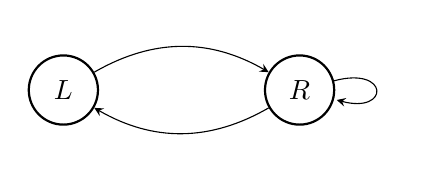
\begin{tikzpicture}[
    node distance=3cm,
    every state/.style={thick},
    ->,
    >=stealth
]

\node[state] (L) {$L$};
\node[state] (R) [right of=L] {$R$};

\draw (L) edge[bend left] node[above] {} (R);
\draw (R) edge[bend left] node[below] {} (L);
\draw (R) edge[loop right] node[right] {} (R);

\end{tikzpicture}

\noindent
The idea is to construct a point of period $k$ by making an orbit like
\[
\underbrace{R\ R\ R\ \cdots\ R}_{k-1}\ L
\]
which follows from the graph.

\noindent \textbf{Construction:}
\begin{align*}
I_0 &= R \\
f^{-1}(I_0) \cap R &\supset I_1 \subset R \\
f^{-1}(I_1) \cap R &\supset I_2 \subset R \\
f^{-1}(I_2) \cap L &\supset I_3 \subset R \\
f^{-3}(I_0) & \quad \text{contraction} \implies \text{must be a fixed point} \\
& \quad \text{(contraction mapping thm)}
\end{align*}

\subsection*{Sharkovskii Ordering of $\mathbb{N}$}
Kinda forgot why we brought this up, but here it is
\[
1 \triangleleft 2 \triangleleft 4 \triangleleft 8 \triangleleft \cdots \triangleleft 2^k \triangleleft \cdots
\]
\[
\cdots \triangleleft 2^2 \cdot 7 \triangleleft 2^2 \cdot 5 \triangleleft 2^2 \cdot 3
\]
\[
\cdots \triangleleft 2 \cdot 7 \triangleleft 2 \cdot 5 \triangleleft 2 \cdot 3
\]
\[
\cdots \triangleleft 7 \triangleleft 5 \triangleleft 3
\]


\subsection{A theorem!}

\underline{Theorem}: If $f$ is continuous and has a period-p orbit, then $f$ has orbits of period $q$ for all $q\triangleleft p$.



\end{document}